% Document format :
\documentclass[12pt,a4paper]{article}
%\usepackage[french]{babel}
\usepackage[english]{babel}
\usepackage[a4paper,left=1.5cm,right=1.5cm,top=2.5cm,bottom=2.5cm]{geometry}
\usepackage{multicol}
\usepackage{indentfirst}
\usepackage[bottom]{footmisc}
\usepackage{fancyhdr}

% Figures :
\usepackage{caption}
\usepackage{subcaption}
\usepackage{graphicx}
\usepackage{float}
\newenvironment{Figure}
{\par\medskip\noindent\minipage{\linewidth}}
{\endminipage\par\medskip}

% Code/Algorithm packages :
\usepackage[table]{xcolor}
\usepackage{listings}
\lstset{
%	linewidth=0.8\columnwidth,
	xleftmargin=0.1\columnwidth,
	xrightmargin=0.1\columnwidth,
	basicstyle=\footnotesize\ttfamily,
	frame=line,
	numbers=left,
	keywordstyle=\color{blue}\bf,
	commentstyle=\color{OliveGreen},
	stringstyle=\color{red},
	breaklines=true,
}
%\lstset{literate=
	%	{á}{{\'a}}1 {é}{{\'e}}1 {í}{{\'i}}1 {ó}{{\'o}}1 {ú}{{\'u}}1
	%	{Á}{{\'A}}1 {É}{{\'E}}1 {Í}{{\'I}}1 {Ó}{{\'O}}1 {Ú}{{\'U}}1
	%	{à}{{\`a}}1 {è}{{\`e}}1 {ì}{{\`i}}1 {ò}{{\`o}}1 {ù}{{\`u}}1
	%	{À}{{\`A}}1 {È}{{\'E}}1 {Ì}{{\`I}}1 {Ò}{{\`O}}1 {Ù}{{\`U}}1
	%	{ä}{{\"a}}1 {ë}{{\"e}}1 {ï}{{\"i}}1 {ö}{{\"o}}1 {ü}{{\"u}}1
	%	{Ä}{{\"A}}1 {Ë}{{\"E}}1 {Ï}{{\"I}}1 {Ö}{{\"O}}1 {Ü}{{\"U}}1
	%	{â}{{\^a}}1 {ê}{{\^e}}1 {î}{{\^i}}1 {ô}{{\^o}}1 {û}{{\^u}}1
	%	{Â}{{\^A}}1 {Ê}{{\^E}}1 {Î}{{\^I}}1 {Ô}{{\^O}}1 {Û}{{\^U}}1
	%	{ã}{{\~a}}1 {ẽ}{{\~e}}1 {ĩ}{{\~i}}1 {õ}{{\~o}}1 {ũ}{{\~u}}1
	%	{Ã}{{\~A}}1 {Ẽ}{{\~E}}1 {Ĩ}{{\~I}}1 {Õ}{{\~O}}1 {Ũ}{{\~U}}1
	%	{œ}{{\oe}}1 {Œ}{{\OE}}1 {æ}{{\ae}}1 {Æ}{{\AE}}1 {ß}{{\ss}}1
	%	{ű}{{\H{u}}}1 {Ű}{{\H{U}}}1 {ő}{{\H{o}}}1 {Ő}{{\H{O}}}1
	%	{ç}{{\c c}}1 {Ç}{{\c C}}1 {ø}{{\o}}1 {å}{{\r a}}1 {Å}{{\r A}}1
	%	{€}{{\euro}}1 {£}{{\pounds}}1 {«}{{\guillemotleft}}1
	%	{»}{{\guillemotright}}1 {ñ}{{\~n}}1 {Ñ}{{\~N}}1 {¿}{{?`}}1 {¡}{{!`}}1 
	%}

% Other packages :
\usepackage{tcolorbox}
\usepackage[hidelinks]{hyperref}


%%%%%%%%%%%%%%%%%%%%%%%%%%%%%%%%%%%%%%%%%%%%%%%%%%%%%%%%%%%%%%%%%%%%%%%%%%%%%%%%%%%%%%%%%%%%%%%%%%%%%%%%%%%%%

\pagestyle{fancy}
%Advanced Algorithmics and Programming -- Models Methods and Programming}
\fancyhead[C]{\footnotesize{\textsc{Advanced Algorithmics and Programming -- Models Methods and Programming}}}
\fancyhead[L]{
\includegraphics[height=1.5em]{img/NU_logo.png}}
\fancyhead[R]{\footnotesize{\textbf{M2BB}}}


%%%%%%%%%%%%%%%%%%%%%%%%%%%%%%%%%%%%%%%%%%%%%%%%%%%%%%%%%%%%%%%%%%%%%%%%%%%%%%%%%%%%%%%%%%%%%%%%%%%%%%%%%%%%%


\begin{document}
	
\title{Multiple Sequence Alignment Project}
\author{Damien \textsc{Garcia} -- Florian \textsc{Echelard}}
\date{January 2023}

\begin{tcolorbox}
	\maketitle
\end{tcolorbox}

\tableofcontents
\listoffigures
\listoftables
	
\thispagestyle{empty}
\pagebreak

%%%%%%%%%%%%%%%%%%%%%%%%%%%%%%%%%%%%%%%%%%%%%%%%%%%%%%%%%%%%%%%%%%%%%%%%%%%%%%%%%%%%%%%%%%%%%%%%%%%%%%%%%%%%%

\section{Compilation and execution}

In order to facilitate usage of the program, a Makefile is provided in the projects archive allowing for easy compilation of the diverse programs:
\begin{itemize}
	\item {\fontfamily{qcr}\selectfont{\textbf{make all}}} : Compiles the complete project.
	\item {\fontfamily{qcr}\selectfont{\textbf{make clean}}} : Removes all the compiled files and potential precompiled headers.
	\item {\fontfamily{qcr}\selectfont{\textbf{make rebuild}}} : Combination of {\fontfamily{qcr}\selectfont{\textbf{make clean}}} and {\fontfamily{qcr}\selectfont{\textbf{make all}}}
	\item {\fontfamily{qcr}\selectfont{\textbf{make data\_generation}}} : Compiles the traces generation program.
	\item {\fontfamily{qcr}\selectfont{\textbf{make alignment}}} : Compiles the alignment program.
	\item {\fontfamily{qcr}\selectfont{\textbf{make quality\_analysis}}} : Compiles the scoring program.
\end{itemize}

Six example are at disposal to test the program and check the execution process.
The program runs syntaxic and semantic checks on the expression to avoid errors and unpredictable behavior during traces generation.
Working examples and basic syntaxic/semantic error case can be executed with the commands:
\begin{itemize}
	\item {\fontfamily{qcr}\selectfont{\textbf{make test\_simple}}} : Working trace generation using simple generative regions.
	\item {\fontfamily{qcr}\selectfont{\textbf{make test\_complex}}} : Working trace generation using complex generative regions.
	\item {\fontfamily{qcr}\selectfont{\textbf{make test\_semantic[1-4]}}} : Execution returns syntaxic and semantic errors handled by the data\_generation program\footnote{{\fontfamily{qcr}\selectfont{make test\_semantic4}} is currently not working. In theory it should return an error, yet it generates traces.}.
\end{itemize}


Each section of the project can be executed independently with the same command line structure: {\fontfamily{qcr}\selectfont{\textbf{./main [inputFile] [outputFile]}}}.
Input file is either the parameters file for the data\_generation program, the traces to align for the alignment program, or the aligned traces for the quality\_analysis program.
Output file is the path where the results should be written.\\

A Python3 script is also at disposal for easy and efficient complete execution of the project.
Use the command: {\fontfamily{qcr}\selectfont{\textbf{python3 pipeline.py [pathToDatasetDirectory]}}}.
The pipeline will handle any necessary compilation, execute the program accordingly to previously explained process and create the results directories if necessary.


%%%%%%%%%%%%%%%%%%%%%%%%%%%%%%%%%%%%%%%%%%%%%%%%%%%%%%%%%%%%%%%%%%%%%%%%%%%%%%%%%%%%%%%%%%%%%%%%%%%%%%%%%%%%%


\section{Traces generation}

The first section of the project aims to generate sequences called traces which are composed of tops and events.
Events can be anchors, meaning they are shared by all generated traces and only exist once for each trace, or simple events that depending on the generation parameters, either exist in a trace or not, and could in some cases have repetitions.
For easier further analysis of the traces, tops are represented by a dot (``."), events always start by a full case ``E" for anchors and lower case ``e" for other events.\\

In order to generate traces, the program relies on parameters files providing a RegEx-like\footnote{Regular Expression} sequence, the number of traces to generate and the maximal size of the traces to generate.

\begin{lstlisting}[caption={Parameter file structure}]
# GENERATION PARAMETERS
expression=(2-3)E1<(4-8)e2X10|E2%25>E2(2-4)E3<(2-5)e1%40>
number_of_traces=20
maximum_length=100
\end{lstlisting}

The expression is separated in 3 sections types :
\begin{itemize}
	\item Simple generative regions : Containing only tops, delimited by parenthesis.
	\item Complex generative regions : Containing tops and events, delimited by a less-than and greater-than signs.
	\item Anchors : Events outside of generative regions.
\end{itemize}

\begin{table}[H]
	\begin{center}
		\caption{Generative regions format}
		\begin{tabular}{|c|ccccccccccccc|}
			\hline
			\textbf{Expression} & $<$ & ( & min & - & max & ) & + & event & X & val & $|$ & ... & $>$ \\
			\hline
			\textbf{Required for simple generation} && \cellcolor{gray} & \cellcolor{gray} & \cellcolor{gray} & \cellcolor{gray} & \cellcolor{gray} &&&&&&& \\
			\hline
			\textbf{Required for complex generation} & \cellcolor{gray} & \cellcolor{gray} & \cellcolor{gray} & \cellcolor{gray} & \cellcolor{gray} & \cellcolor{gray} && \cellcolor{gray} &&&&& \cellcolor{gray} \\
			\hline
		\end{tabular}
	\end{center}
\end{table}

Traces are generated and written in a single file, with on expression per line as seen below.

\begin{lstlisting}[caption={Traces generated from expression (2-3)E1$<$(4-8)e2X10$|$E2\%25$>$E2(2-4)E3$<$(2-5)e1\%40$>$}]
. . . . E1 . e2 . e2 E2 . . . . . E3 . . . . .
. . E1 . . e2 e2 . e2 . . E2 . . E3 e1 . e1 e1 e1
. . E1 . . . . . . . E2 . . . . . E3 . e1 e1
. . . . E1 e2 . e2 . . . . E2 . . E3 . . . . . .
. . . . E1 e2 . e2 . E2 . . . . . E3 . . .
. . . E1 . . . . . . . . . . . E2 . . . . . E3 . .
. . . E1 . . . e2 . . e2 . . E2 . . . . E3 . . . . .
. . . . E1 . . e2 e2 . . . . . E2 . . . E3 . e1
. . E1 . e2 . . . e2 E2 . . E3 . . . e1
. . E1 . . . . . . . . E2 . . E3 . e1 .
. . . . E1 e2 . . . . . . e2 . . E2 . . E3 . . . . .
. . E1 . . . . . E2 . . . . . E3 . e1
. . . E1 . . . . . . . . E2 . . . . . E3 . . .
. . E1 e2 e2 . . . . . . E2 . . E3 . .
. . E1 . . . . . . E2 . . . . E3 . e1 . e1 e1 e1
. . . . E1 . . . . . . . E2 . . . . . E3 . e1 e1
. . . . E1 e2 . . . . . E2 . . . . . E3 . . .
. . . E1 . . . . . . e2 E2 . . E3 . . . .
. . . E1 e2 . e2 e2 E2 . . . . . E3 . . .
. . . E1 . . e2 e2 e2 . . . E2 . . E3 . .
\end{lstlisting}


%%%%%%%%%%%%%%%%%%%%%%%%%%%%%%%%%%%%%%%%%%%%%%%%%%%%%%%%%%%%%%%%%%%%%%%%%%%%%%%%%%%%%%%%%%%%%%%%%%%%%%%%%%%%%


\section{Multiple Sequence Alignment (MSA)}


To perform the MSA, the program relies on two main methods being (i) pairwise alignment algorithm and (ii) Unweighted Pair Group Method with Arithmetic mean (UPGMA) algorithm.
The decision guiding the order in which traces will be aggregated by UPGMA algorithm is by measuring the dissimilarity between each pair of traces. This measure is inherently linked to the pairwise alignment process.

\begin{itemize}
\item[\textbf{Step 1}] At first, all the traces are stored into a data type that can either contain one or more traces.
This way, when a pair of traces will be aggregated, the algorithm won't have to rely on different methods and functions depending on the progress of the MSA.
All functions and methods are programmed to process two single traces as well as batches of traces.

\item[\textbf{Step 2}] Next, every pair is aligned which allows to get the dissimilarity score.
The pair with the lowest dissimilarity score is then selected and modified with considerations to the alignment results.
At this point the traces might include gaps represented by hyphens (``-'').
The updated traces are then aggregated into one batch of traces.

\item[\textbf{Step 3}] The dissimilarity matrix\footnote{Represented by a lower triangular matrix for optimization purpose. $Dissim(T1, T2) = Dissim(T2, T1)$} is updated by removing the pairs and adding the new batch of traces.
The dissimilarity score for the new batch is then calculated with every other traces and/or batches.
This method allows the algorithm to avoid recalculating every dissimilarity score by keeping unmodified data and only calculating scores for new batches.
\end{itemize}

\textbf{Steps 2} and \textbf{3} are repeated until all traces are aggregated into one batch.

\begin{figure}[H]
	\begin{subfigure}[t]{0.33\linewidth}
		\centering
		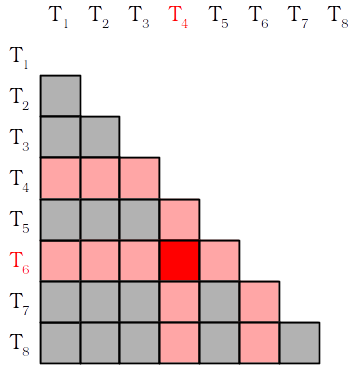
\includegraphics[width=0.8\linewidth]{img/matrix1.png}
		\caption{}
		\label{sub:matrix1}
	\end{subfigure}
	\begin{subfigure}[t]{0.33\linewidth}
		\centering
		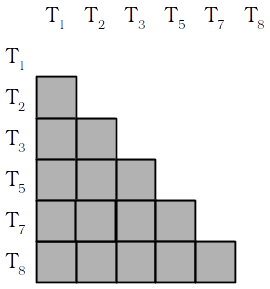
\includegraphics[width=0.6\linewidth]{img/matrix2.png}
		\caption{}
		\label{sub:matrix2}	
	\end{subfigure}
	\begin{subfigure}[t]{0.33\linewidth}
		\centering
		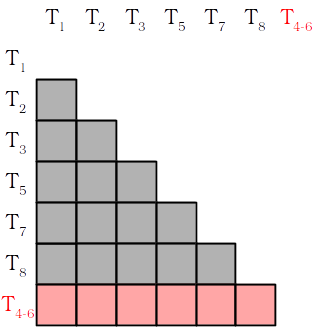
\includegraphics[width=0.7\linewidth]{img/matrix3.png}
		\caption{}
		\label{sub:matrix3}
	\end{subfigure}
	\caption{Dissimilarity matrix update}{
		\emph{\color{blue}{(a)}} Selection of minimum dissimilarity (red cell) and removing the values from the corresponding traces (pink cells).
		\emph{\color{blue}{(b)}} Resulting matrix after step \emph{\color{blue}{a}}.
		\emph{\color{blue}{(c)}} Adding aggregated traces and performing dissimilarity calculations for the new cells.
	}
	\label{fig:matrix}
\end{figure}


%%%%%%%%%%%%%%%%%%%%%%%%%%%%%%%%%%%%%%%%%%%%%%%%%%%%%%%%%%%%%%%%%%%%%%%%%%%%%%%%%%%%%%%%%%%%%%%%%%%%%%%%%%%%%


\section{MSA quality assessment}

\subsection{Scoring functions}

\subsection{Quality of the method}



%%%%%%%%%%%%%%%%%%%%%%%%%%%%%%%%%%%%%%%%%%%%%%%%%%%%%%%%%%%%%%%%%%%%%%%%%%%%%%%%%%%%%%%%%%%%%%%%%%%%%%%%%%%%%


\section{Prospects}

As seen by the various results presented, the alignment is of relatively good quality considering the questionable methods used in the algorithm.

The main concern is that the values for indel\footnote{Insertions and deletions} and substitutions are fixed \emph{a priori} while these weights could be carefully chosen based on the inputs.
For example, with batches of traces showing large difference between lengths, the number of gaps introduced will accordingly be higher than in an ideal case.
Therefor, lowering the cost of gaps in comparison to the cost of mismatches on events should allow for wider gaps and align tops and events.
Another way of solving this problem could be to lower the cost of gap introduction around other gaps, also resulting in wider gaps segments and better alignment of tops and events.

The second concern is that this algorithm aims to align traces which have no actual real life meaning.
The traces could be the reflection of time series, genes recognition in a sequencing process, or any other situation.
Adding context around these traces would allow for revisions on the alignment process.

\pagebreak


%%%%%%%%%%%%%%%%%%%%%%%%%%%%%%%%%%%%%%%%%%%%%%%%%%%%%%%%%%%%%%%%%%%%%%%%%%%%%%%%%%%%%%%%%%%%%%%%%%%%%%%%%%%%%


\section*{Supplementary material}
\addcontentsline{toc}{section}{Supplementary material}

\noindent\footnotesize{\textbf{Code accessible on GitHub repository:}
\href{https://github.com/Damien-Garcia-Bioinformatics/aap\_mma\_project}{\color{blue}{https://github.com/Damien-Garcia-Bioinformatics/aap\_mma\_project}}}

\begin{figure}[H]
	\centering
	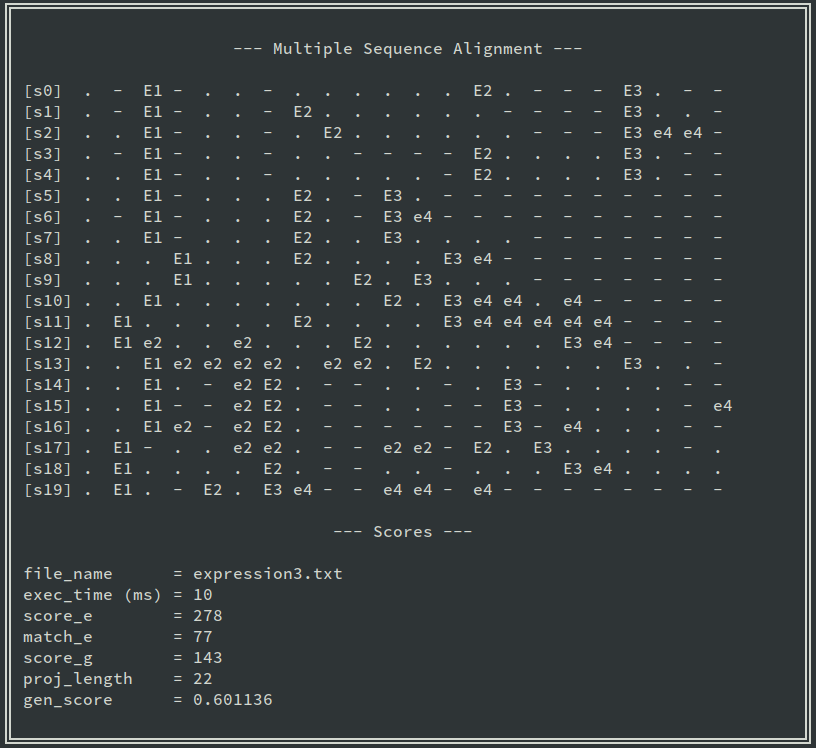
\includegraphics[width=0.75\linewidth]{img/terminal_output.png}
	\caption{Terminal output from python pipeline}
	\label{fig:output}
\end{figure}

\begin{figure}[H]
	\centering
	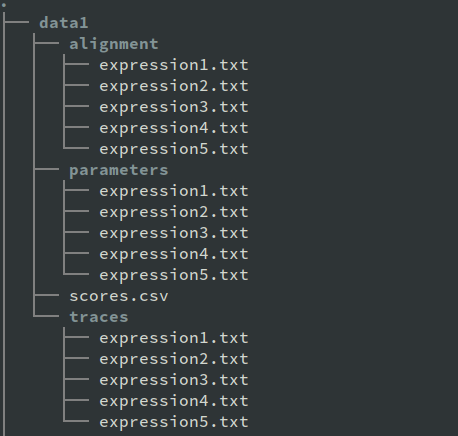
\includegraphics[width=0.45\linewidth]{img/terminal_tree.png}
	\caption{Terminal output from python pipeline}
	\label{fig:tree}
\end{figure}


\pagebreak


\begin{table}[H]
	\begin{center}
		\caption{Dataset 1 scoring results}
		\begin{tabular}{|c|c|c|c|c|c|c|}
			\hline
			\textbf{file\_name} & \textbf{exec\_time} (ms) & \textbf{score\_e} & \textbf{match\_e} & \textbf{score\_g} & \textbf{proj\_length} & \textbf{general\_score} \\
			\hline\hline
			expression1.txt & 13 & 462 & 58 & 194 & 33 & 0.659394 \\
			\hline
			expression2.txt & 40 & 812 & 79 & 425 & 62 & 0.623629 \\
			\hline
			expression3.txt & 20 & 589 & 55 & 185 & 39 & 0.703333 \\
			\hline
			expression4.txt & 12 & 427 & 78 & 188 & 31 & 0.650161 \\
			\hline
			expression5.txt & 28 & 726 & 53 & 267 & 50 & 0.680100 \\
			\hline
		\end{tabular}
	\end{center}
\end{table}

\begin{table}[H]
	\begin{center}
		\caption{Dataset 2 scoring results}
		\begin{tabular}{|c|c|c|c|c|c|c|}
			\hline
			\textbf{file\_name} & \textbf{exec\_time} (ms) & \textbf{score\_e} & \textbf{match\_e} & \textbf{score\_g} & \textbf{proj\_length} & \textbf{general\_score} \\
			\hline\hline
			expression1.txt & 19 & 405 & 103 & 202 & 31 & 0.620484 \\
			\hline
			expression2.txt & 15 & 399 & 109 & 130 & 27 & 0.689074 \\
			\hline
			expression3.txt & 10 & 278 & 77  & 143 & 22 & 0.601136 \\
			\hline
			expression4.txt & 27 & 580 & 138 & 154 & 37 & 0.726216 \\
			\hline
			expression5.txt & 16 & 451 & 80  & 164 & 31 & 0.681129 \\
			\hline
		\end{tabular}
	\end{center}
\end{table}

\begin{table}[H]
	\begin{center}
		\caption{Dataset 3 scoring results}
		\begin{tabular}{|c|c|c|c|c|c|c|}
			\hline
			\textbf{file\_name} & \textbf{exec\_time} (ms) & \textbf{score\_e} & \textbf{match\_e} & \textbf{score\_g} & \textbf{proj\_length} & \textbf{general\_score} \\
			\hline\hline
			expression1.txt & 104 & 1169 & 180 & 644 & 93  & 0.600269 \\
			\hline
			expression2.txt & 215 & 1615 & 401 & 513 & 108 & 0.696667 \\
			\hline
			expression3.txt & 275 & 1847 & 487 & 495 & 119 & 0.719244 \\
			\hline
			expression4.txt & 17  & 459  & 103 & 126 & 30  & 0.709500 \\
			\hline
			expression5.txt & 14  & 459  & 108 & 152 & 31  & 0.690806 \\
			\hline
		\end{tabular}
	\end{center}
\end{table}

\begin{table}[H]
	\begin{center}
		\caption{Dataset 4 scoring results}
		\begin{tabular}{|c|c|c|c|c|c|c|}
			\hline
			\textbf{file\_name} & \textbf{exec\_time} (ms) & \textbf{score\_e} & \textbf{match\_e} & \textbf{score\_g} & \textbf{proj\_length} & \textbf{general\_score} \\
			\hline\hline
			expression1.txt & 58 & 933 & 176 & 386 & 67 & 0.655448 \\
			\hline
			expression2.txt & 44 & 779 & 186 & 383 & 59 & 0.626610 \\
			\hline
			expression3.txt & 27 & 628 & 152 & 206 & 42 & 0.697381 \\
			\hline
			expression4.txt & 27 & 626 & 142 & 258 & 45 & 0.654667 \\
			\hline
			expression5.txt & 48 & 885 & 157 & 176 & 54 & 0.753796 \\
			\hline
		\end{tabular}
	\end{center}
\end{table}


\pagebreak


\begin{figure}[H]
	\begin{subfigure}[t]{0.5\linewidth}
		\centering
		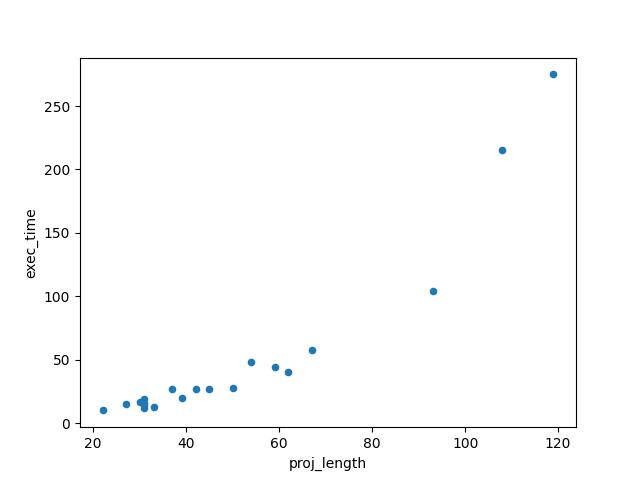
\includegraphics[width=1\linewidth]{plots/lenVStime.jpg}
		\caption{graph1}
		\label{sub:graph1}
	\end{subfigure}
	\begin{subfigure}[t]{0.5\linewidth}
		\centering
		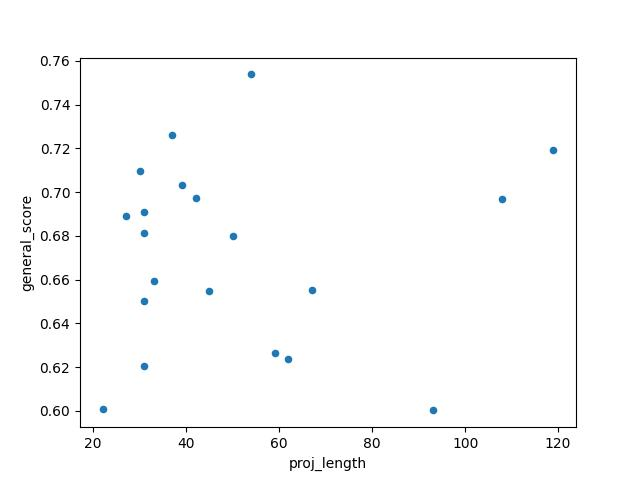
\includegraphics[width=1\linewidth]{plots/lenVSgen.jpg}
		\caption{graph2}
		\label{sub:graph2}	
	\end{subfigure}
	\begin{subfigure}[t]{0.5\linewidth}
		\centering
		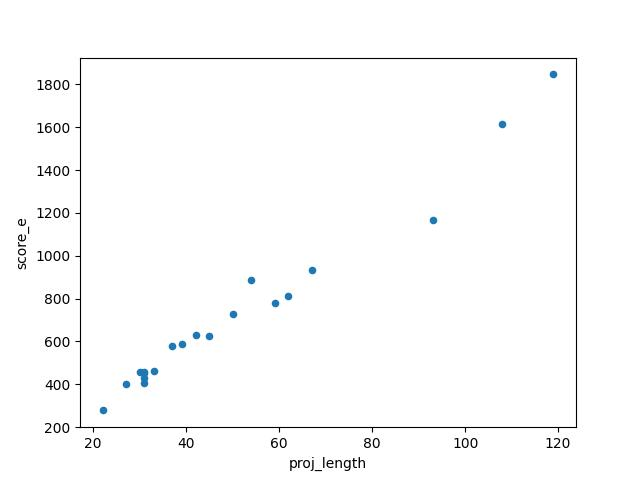
\includegraphics[width=1\linewidth]{plots/lenVSse.jpg}
		\caption{graph3}
		\label{sub:graph3}
	\end{subfigure}
	\begin{subfigure}[t]{0.5\linewidth}
		\centering
		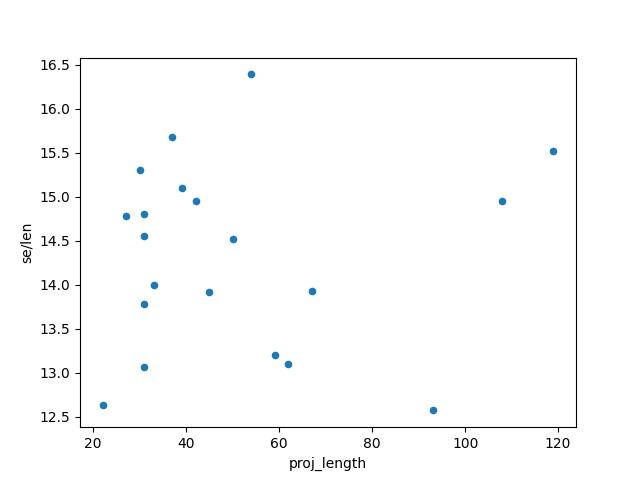
\includegraphics[width=1\linewidth]{plots/lenVSselen.jpg}
		\caption{graph4}
		\label{sub:graph4}	
	\end{subfigure}
		\begin{subfigure}[t]{0.5\linewidth}
		\centering
		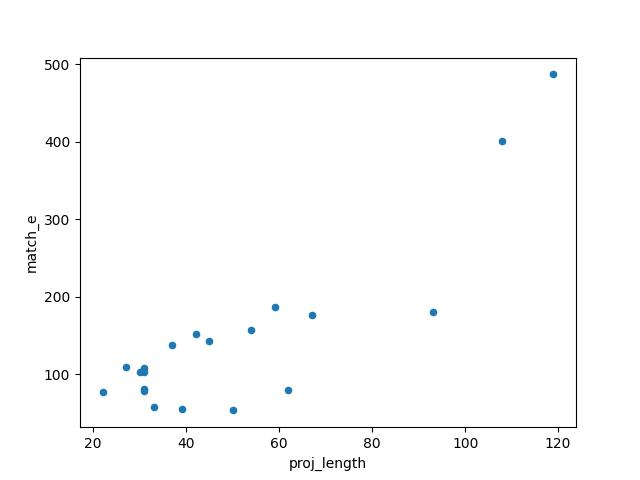
\includegraphics[width=1\linewidth]{plots/lenVSme.jpg}
		\caption{graph5}
		\label{sub:graph5}
	\end{subfigure}
	\begin{subfigure}[t]{0.5\linewidth}
		\centering
		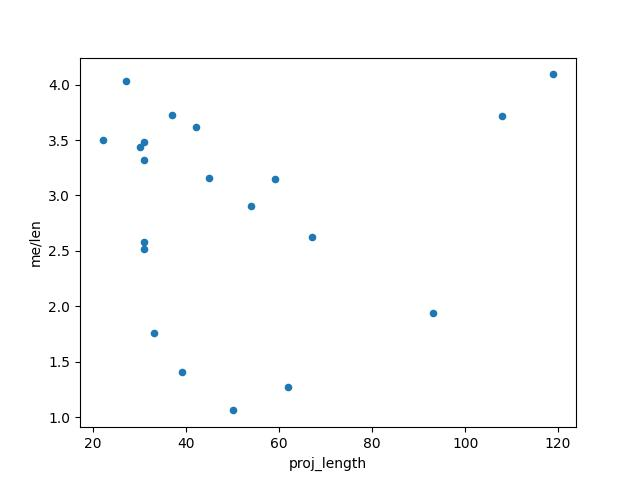
\includegraphics[width=1\linewidth]{plots/lenVSmelen.jpg}
		\caption{graph6}
		\label{sub:graph6}	
	\end{subfigure}
	\caption{blabla}
	\label{fig:graphs}
\end{figure}


\end{document}